% vim: textwidth=78 ai

\appendix
  \chapter{Udev files}
  \label{app.udev}
  Commented file listings of udev rules and a script which is called from
  those rules are following.

  \section{udev rules file}
\begin{lstlisting}[language={},label=lst.udevrules,name=lst.udevrules]
KERNEL!="combosix*", GOTO="cesnet_generator_end"(*@\label{lstl.udevrules_1}@*)
ACTION!="add", GOTO="cesnet_generator_end"(*@\label{lstl.udevrules_2}@*)
NAME=="?*", GOTO="cesnet_generator_end"(*@\label{lstl.udevrules_3}@*)
\end{lstlisting}
  Since we want to match only additions of combosix devices, rules at line
  \ref{lstl.udevrules_1} and \ref{lstl.udevrules_2} are needed. To ignore
  cases where the stored name was set yet, the skip rule at line
  \ref{lstl.udevrules_3} is there.
\begin{lstlisting}[name=lst.udevrules]
ENV{CS}="$kernel"
ENV{MATCHPATH}="$devpath"
\end{lstlisting}
  Set up environment variables used in shell script later. These variables are
  filled in directly by \emph{udev} and corresponds to the name suggested by
  kernel or device path (i.e. bus, slot\ldots) respectively.
\begin{lstlisting}[name=lst.udevrules]
IMPORT{PROGRAM}="csdevname" (*@\label{lstl.udevrules_11}@*)

ENV{CS_NEW}=="?*", NAME="$env{CS_NEW}"

LABEL="cesnet_generator_end" (*@\label{lstl.udevrules_12}@*)
\end{lstlisting}
  And finally invoke the script and set up the new name if the script changed
  it. The last step (line \ref{lstl.udevrules_12}) is to define a label where
  the first 3 rules jump to.

  \section{csdevname script}
  Shell script \textbf{csdevname} called from line \ref{lstl.udevrules_11}
  above follows:
\lstset{language=bash} % XXX TODO
\begin{lstlisting}[label=lst.udevscript,name=lst.udevscript]
RULES_FILE='/etc/udev/rules.d/70-cesnet.rules'

. /lib/udev/rule_generator.functions(*@\label{lstl.udevscript_1}@*)
\end{lstlisting}
  This loads udev predefined functions used later. RULES\_FILE is the
  name of file, where we store our persistent naming. Variable name is
  predefined (and used in the script sourced at line \ref{lstl.udevscript_1})
  and must not be changed.
\begin{lstlisting}[name=lst.udevscript]
cs_name_taken() {
	local value="$(find_all_rules 'NAME=' $CS)"
	if [ "$value" ]; then return 0; else return 1; fi
}

find_next_available() {
	raw_find_next_available "$(find_all_rules 'NAME=' "$1")"
}
\end{lstlisting}
  Functions \textbf{cs\_name\_taken} and \textbf{find\_next\_available} are
  for finding available names for new coming device. Both uses functions
  defined in the sourced script from line \ref{lstl.udevscript_1}, that allows
  be them as compact as possible.
\begin{lstlisting}[name=lst.udevscript]
write_rule() {
	local match="$1"
	local name="$2"
	local comment="$3"
	{
		[ "$comment" ] && echo "# $comment"
		echo "SUBSYSTEM==\"combosix\", ACTION==\"add\"$match, NAME=\"$name\""
	} >> $RULES_FILE
}
\end{lstlisting}
  \textbf{write\_rule} takes 3 parameters -- under which condition this rule
  is triggered, static node name and potentially a comment to this rule. The
  result is written to previously defined \textbf{RULES\_FILE}.
\begin{lstlisting}[name=lst.udevscript]
lock_rules_file(*@\label{lstl.udevscript_27}@*)
choose_rules_file(*@\label{lstl.udevscript_29}@*)
\end{lstlisting}
  At lines \ref{lstl.udevscript_27} and \ref{lstl.udevscript_29} we lock up
  the rules file to prevent race
  conditions (if two writers occurred, it would result in unpredictable
  behavior) and decide in which file will be the new rules written (since
  usual location might be still read-only while booting -- \emph{udev} will
  then move the temporary file to the proper directory after it becomes
  writable).
\begin{lstlisting}[name=lst.udevscript]
MATCHPATH=${MATCHPATH%/*/*}
if [ "$MATCHPATH" ]; then
	match="$match, DEVPATH==\"$MATCHPATH/*\""
fi

if [ -z "$match" ]; then
	echo "missing valid match" >&2
	unlock_rules_file
	exit 1
fi
\end{lstlisting}
  Now we define matching rule passed to \textbf{write\_rule} later (line
  \ref{lstl.udevscript_49}). Sanity check of the value is done here and if it
  fails we return error.
\begin{lstlisting}[name=lst.udevscript]
if [ "$CS_NAME" ]; then
	COMMENT="$COMMENT (custom name)"
	if [ "$CS_NAME" != "$CS" ]; then
		CS=$CS_NAME;
		echo "CS_NEW=$CS"
	fi
else
	base=${CS%%[0-9]*}
	if cs_name_taken; then
		CS="$base$(find_next_available "$base[0-9]*")"
		echo "CS_NEW=$CS"
	fi
fi
\end{lstlisting}
  Here the name, which is returned to rules (\textbf{CS\_NEW}), is set. Logic
  is simple, either the one passed by external application is used or a new
  one is found (first unused).
\begin{lstlisting}[name=lst.udevscript]
write_rule "$match" "$CS" "$COMMENT"(*@\label{lstl.udevscript_49}@*)

unlock_rules_file
\end{lstlisting}
  Finally the file with static naming is augmented and unlocked.

  Since this moment, if the device come in the system again later, even in
  other order, system will ever create a node with the same name loaded from
  the rules file.
\chapter{Models}
  \label{app.models}
  Here comes the models of the design and the description (the one generated
  from bouml).

  \newpage
  \begin{center}
    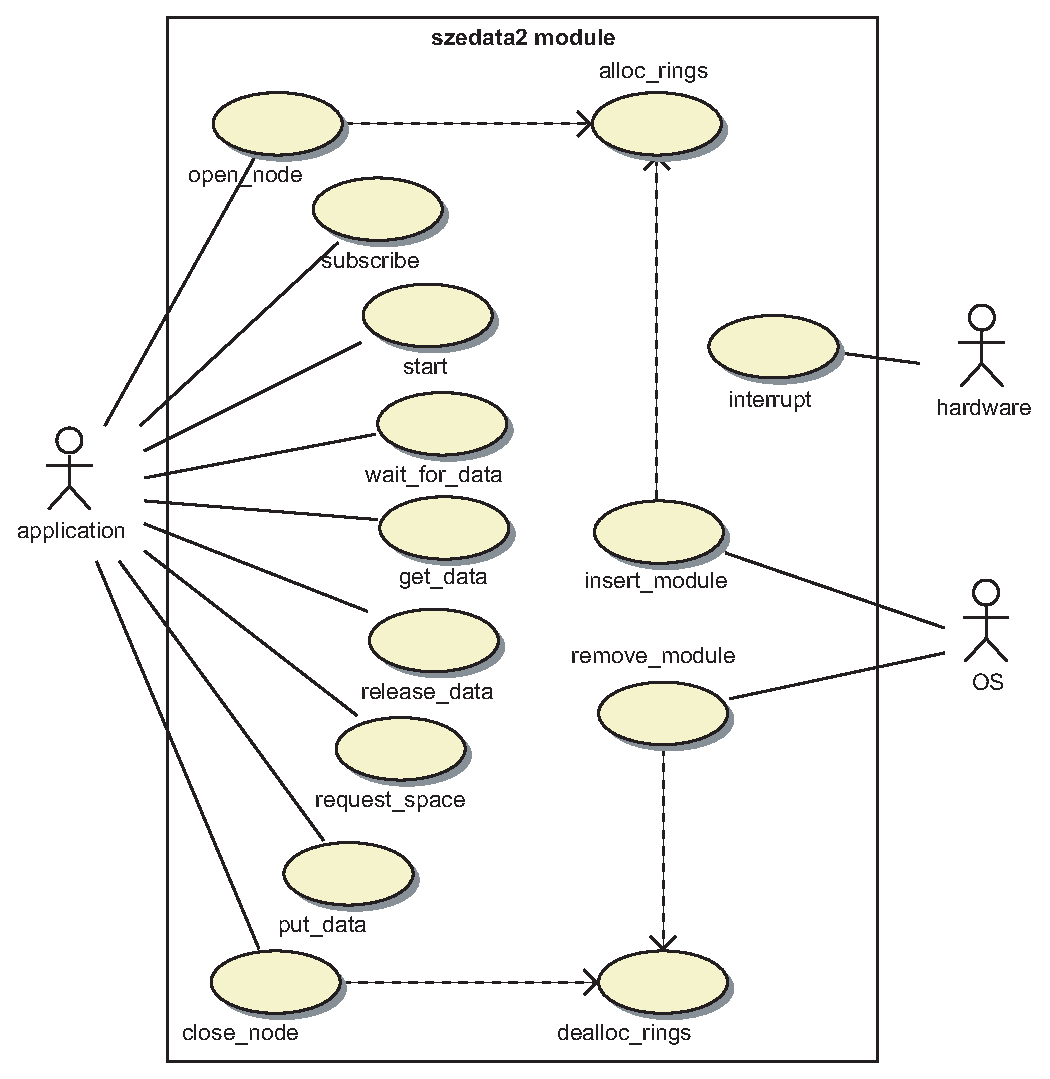
\includegraphics[width=12.5cm]{images/usecase}
  \end{center}

  \newpage
  \begin{center}
    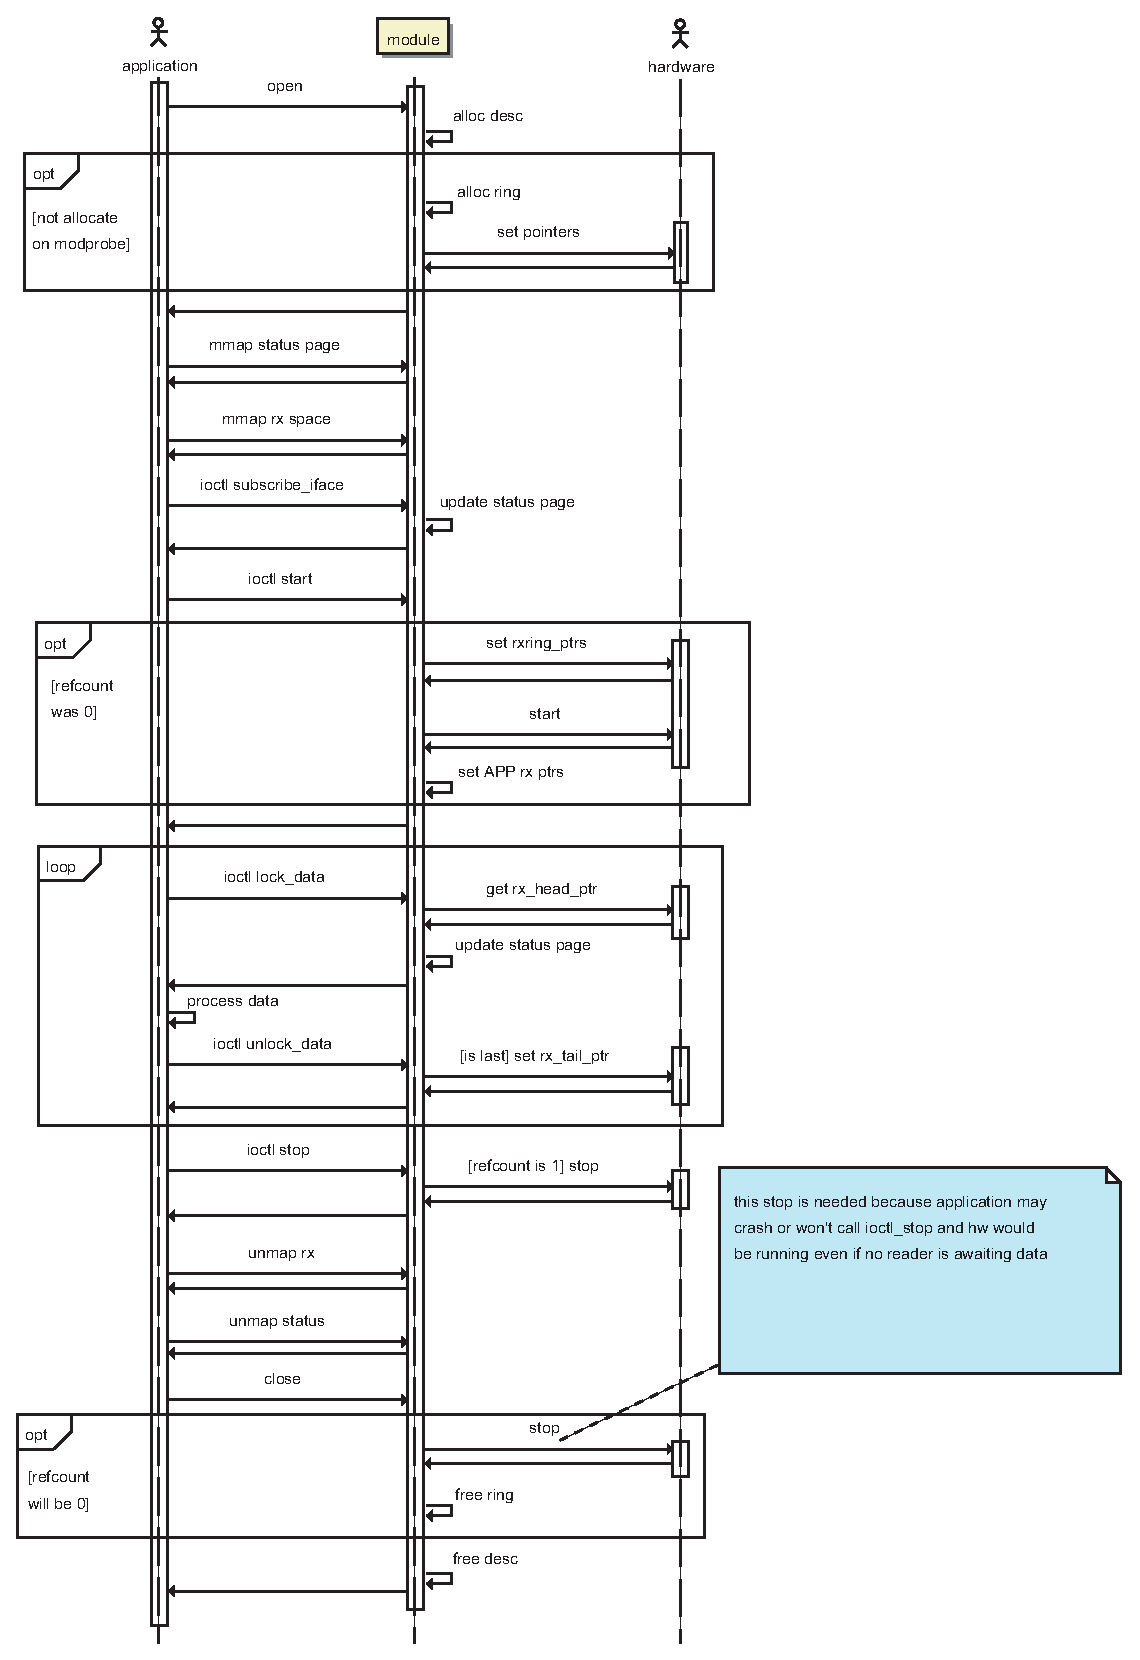
\includegraphics[width=12.5cm]{images/seqd_rx}
  \end{center}

  \newpage
  \begin{center}
    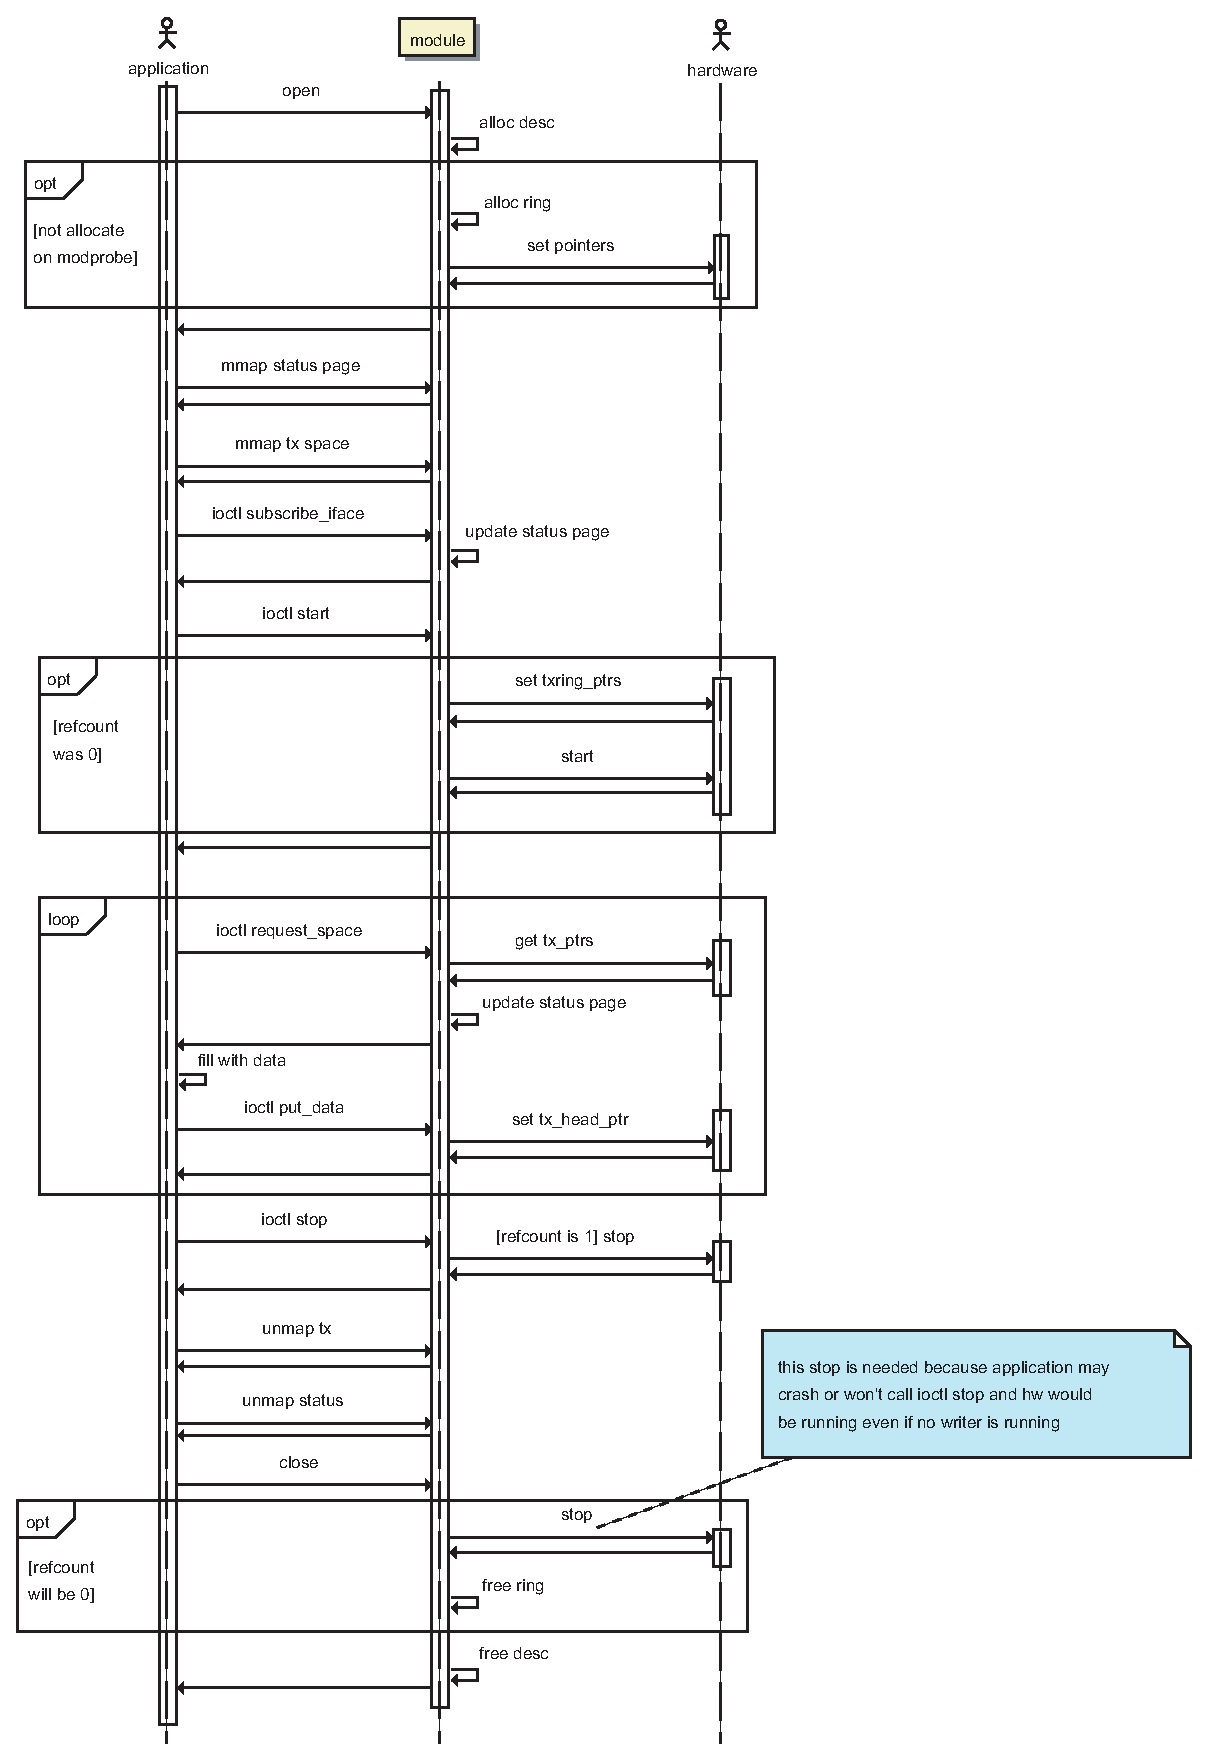
\includegraphics[width=12.5cm]{images/seqd_tx}
  \end{center}

\chapter{Documentation}
  Probably generated doxygen docs and wiki pages with short user's manual.
